%\section{Introduction}
%TBD
%\newpage

\section{Glossary}

The following terms are used frequently throughout this document:

\begin{itemize}
    \item \textbf{dkey} - A DAOS 'distribution key,' which denotes a set of arrays co-located on the same storage targets. A dkey has an arbitrary size.
    \item \textbf{akey} - A DAOS 'attribute key,' which distinguishes individual arrays. Similar to a dkey, an akey has an arbitrary size.
\end{itemize}

\newpage

\section{VOL Connector Design}

\subsection{Mapping HDF5 to DAOS}

The central paradigm for mapping HDF5 to DAOS is that HDF5 files are stored as DAOS containers, and HDF5 objects (groups, datasets, committed datatypes, and maps) are stored as DAOS objects, both using a 1:1 mapping. All metadata and raw data associated with an HDF5 object is then stored as entries in the key value store associated with that object provided by DAOS.

Since DAOS containers are identified by a UUID, the connector uses a hashing function to generate a UUID from the file name. Each container for an HDF5 file contains at least two objects: the global metadata object and the root group. The global metadata object stores metadata that describes properties that apply to the entire file. The root group is always the start of the HDF5 group structure, and uses the same format as all other groups.

Similar to the native HDF5 file format, the formats for the different object types are kept similar, with only differences as necessary to represent the specific object type. All object types have a creation property list and a reference count (not yet implemented) stored under the ``/Internal Metadata'' dkey and the ``Creation Property List'' and ``Reference Count'' akeys, respectively. The \verb+/+ prefix for the ``/Internal Metadata'' dkey prevents conflicts with arbitrarily named HDF5 links, which cannot contain the \verb+/+ character.

\newpage

\subsubsection{Groups}

The purpose of HDF5 groups is to store links to other objects. Each link is stored under a dkey equal to the link's name and under the constant akey \verb+Link+. Links can be hard links, in which case the value stored for the link is the object ID for the target object. This object ID can then be used to directly open the target object. Alternatively, links can be soft links, in which case the value stored for the link is the path name of the target object. Once retrieved, this path name must be traversed in order to open the target object.

When link creation order is tracked for a group, additional information is written to that group under the \verb+/Link Creation Order+ dkey. Under that dkey, link creation order-related information is stored under the following akeys:

\begin{itemize}
    \item \verb+Max Link Creation Order+ - This akey stores the current maximum link creation order value for the group. The maximum link creation order value starts at 0 and increases as new links are created in the group. This value is mostly used to supply a group's maximum link creation order value when a call to \verb+H5Gget_info(_by_name/_by_idx)+ is made.
    \item \verb+Num Links+ - This akey stores the current number of links in the group.
    \item \verb+<encoded num. links>+ - The value for this akey is determined by encoding the current number of links in the group \textit{at creation time of the new link} into a binary buffer; this encoded value represents the creation order index value assigned to the new link being written. This akey is used to store a mapping from link creation order index values to link names, which allows an easy lookup of a link's name by a given creation order index value. One of these akeys will exist for each link currently in the group, as a new akey will be added each time a new link is written to the group.
    \item \verb+<encoded num. links>0+ - The value for this akey is determined similarly to the previous akey, but the akey value is suffixed with a trailing \verb+0+ byte in order to distinguish it from the previous akey. This akey is used to store a mapping from link creation order index values to link targets, which allows an easy lookup of a link's target by a given creation order index value. One of these akeys will exist for each link currently in the group, as a new akey will be added each time a new link is written to the group.
\end{itemize}

\todo{Update figure for creation order changes}
\begin{figure}
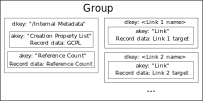
\includegraphics[width=0.6\textwidth]{pics/group_figure}
\caption{Group Dkey and link examples.}
\label{fig:group}
\end{figure}

\newpage

\subsubsection{Datasets}

Datasets are used to store the bulk array data in HDF5. A dataset's metadata is stored under the \verb+/Internal Metadata+ dkey and under the following akeys:

\begin{itemize}
    \item \verb+Datatype+ - This akey stores the dataset's datatype.
    \item \verb+Dataspace+ - This akey stores the dataset's dataspace.
    \item \verb+Creation Property List+ - This akey stores the dataset's Dataset Creation Property List.
\end{itemize}

A dataset's raw data is divided into ``chunks'' which are regularly spaced blocks of data, where the size of the block is specified by the application. Each data chunk is stored in its own dkey, which is encoded with a leading 0 byte, followed by $<$number of dimensions$>$ 64-bit little endian unsigned integers which denote the chunk offset within the dataset. The \verb+0+ prefix for chunks prevents the binary chunk dkeys from conflicting with the string metadata dkeys, since nonzero length strings cannot begin with 0 (\verb+\0+).

For datasets with fixed-length datatypes, the data for a chunk is stored in a single akey with a value of a 0 byte. The data is stored as an array of records, where each record corresponds to an element in the dataset. The record size is therefore equal to the size of the datatype and the number of records is equal to the number of elements in the data chunk. For datasets with variable-length datatypes, each element is stored in a separate akey, and as a single record whose size is equal to the total size of the variable-length element.

\todo{Add figure for variable-length datasets}
\begin{figure}
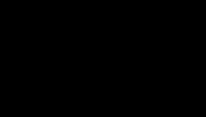
\includegraphics[width=0.6\textwidth]{pics/dataset_figure}
\caption{Fixed Length Dataset Dkey examples.}
\label{fig:dataset}
\end{figure}

\newpage

\subsubsection{Committed Datatypes}

A committed datatype is an HDF5 datatype that has been stored as an HDF5 object in the group structure. A committed datatype's metadata is stored under the \verb+/Internal Metadata+ dkey and under the following akeys:

\begin{itemize}
    \item \verb+Datatype+ - This akey stores the committed datatype's actual datatype.
    \item \verb+Creation Property List+ - This akey stores the committed datatype's Datatype Creation Property List.
\end{itemize}

\todo{Add figure for committed datatype}

\newpage

\subsubsection{Attributes}

HDF5 attributes attached to an object (group, dataset, committed datatype or map object) are stored under that object's \verb+/Attribute+ dkey (note that the \verb+/+ prefix for the \verb+/Attribute+ dkey prevents conflicts with arbitrarily named HDF5 links, which cannot contain the \verb+/+ character). Under that dkey, an attribute's metadata and raw data is stored under the following akeys:

\begin{itemize}
    \item \verb+T-<attribute name>+ - This akey stores the attribute's datatype.
    \item \verb+S-<attribute name>+ - This akey stores the attribute's dataspace.
    \item \verb+P-<attribute name>+ - This akey stores the attribute's Attribute Creation Property List.
    \item \verb+V-<attribute name>+ - This akey stores the attribute's value.
\end{itemize}

When attribute creation order is tracked for an object, additional information is written to that object under the same \verb+/Attribute+ dkey and under the following akeys:

\begin{itemize}
    \item \verb+Max Attribute Creation Order+ - This akey stores the current maximum attribute creation order value for the object. The maximum attribute creation order value starts at 0 and increases as new attributes are added to the object.
    \item \verb+Num Attributes+ - This akey stores the current number of attributes attached to the object.
    \item \verb+0<encoded num. attributes>+ - The value for this akey is determined by encoding the current number of attributes attached to the object \textit{at creation time of the new attribute} into a binary buffer, prefixed with a leading \verb+0+ byte; this encoded value represents the creation order index value assigned to the new attribute being written. This akey is used to store a mapping from attribute creation order index values to attribute names, which allows an easy lookup of an attribute's name by a given creation order index value. One of these akeys will exist for each attribute currently attached to the object, as a new akey will be added each time a new attribute is written to the object.
    \item \verb+C-<attribute name>+ - This akey stores the attribute's creation order value.
\end{itemize}

\todo{Add figure for attributes + attribute creation order}

\newpage

\subsubsection{Object IDs}

\todo{Update for DAOS object ID allocator changes}

DAOS objects are referenced through the DAOS API by a 128 bit object ID. Only the lower 64 bits are currently used by HDF5, the rest of the ID is set to 0 and/or set by DAOS to encode the DAOS object class, which is always the same for each HDF5 object type. The lower 62 bits are simply set in increasing order, starting from 1, which is always the root group (0 is reserved for a global metadata object). The remaining 2 bits are used to encode the HDF5 object type. This
removes the need to store the object type in the key-value store for the object itself, and allows the connector to determine the object type and therefore the routines used to access it without needed to query DAOS, reducing the number of server requests needed for metadata operations. The lower 64 bits (including the encoded object type) are considered the “address” for the purposes of the HDF5 API, and is what is returned as \verb+addr+ from \verb+H5Oget_info()+ and what is accepted for \verb+H5Oopen_by_addr()+.

Object ID allocation is currently not handled correctly when done independently by multiple processes. This is a temporary solution until a DAOS object ID allocator is available. This means that either all objects should be created by the same process, or they should always be created collectively using \verb+H5Pset_all_coll_metadata_ops()+.

\newpage

\section{HDF5 Map Objects}

\todo{Add notes}

While the HDF5 data model is a flexible way to store data that is widely used in HPC, some applications require a more general way to index information. While HDF5 effectively uses key-value stores internally for a variety of purposes, it does not expose a generic key-value store to the API. As part of the DAOS project, we will be adding this capability to the HDF5 API, in the form of HDF5 Map objects. These Map objects will contain application-defined key-value stores, to which key-value pairs can be added, and from which values can be retrieved by key.

\subsection{Map Object API}
To implement map objects, we will add new API routines, and new VOL callbacks, to the HDF5 library. For now, though, we will not be implementing support for maps in the default (native) VOL connector, meaning that map objects will only work with the DAOS connector, and with any other VOL connectors that are written to support maps.

The HDF5 Map API will consist of 11 new HDF5 API functions for managing Map objects, plus closely related functions such as \verb+H5Mcreate_anon()+, \verb+H5Mopen_by_name()+, etc. that are excluded from this list for the sake of brevity.

\subsubsection{H5Mcreate}

{\lstsetc
\begin{lstlisting}
hid_t H5Mcreate(hid_t loc_id, const char *name, hid_t keytype, hid_t valtype, hid_t lcpl_id, hid_t mcpl_id, hid_t mapl_id);
\end{lstlisting}
}

\verb+H5Mcreate()+ creates a new Map object in the specified location in the HDF5 file and with the specified name. The datatype for keys and values can be specified separately, and any further options can be specified through the property lists \verb+lcpl_id+, \verb+mcpl_id+, and \verb+mapl_id+.


\subsubsection{H5Mopen}

{\lstsetc
\begin{lstlisting}
hid_t H5Mopen(hid_t loc_id, const char *name, hid_t mapl_id);
\end{lstlisting}
}

\verb+H5Mopen()+ opens a previously created Map object at the specified location with the specified name. Any further options can be specified through the property list \verb+mapl_id+.

\subsubsection{H5Mput}

{\lstsetc
\begin{lstlisting}
herr_t H5Mput(hid_t map_id, hid_t key_mem_type_id, const void *key, hid_t val_mem_type_id, const void *value, hid_t dxpl_id);
\end{lstlisting}
}

\verb+H5Mput()+ adds a key-value pair to the Map specified by \verb+map_id+, or updates the value for the specified key if one was set previously. \verb+key_mem_type_id+ and \verb+val_mem_type_id+ specify the datatypes for the provided key and value buffers, and if different from those used to create the Map object, the key and value will be internally converted to the datatypes for the map object. Any further options can be specified through the property list \verb+dxpl_id+.

\subsubsection{H5Mget}

{\lstsetc
\begin{lstlisting}
herr_t H5Mget(hid_t map_id, hid_t key_mem_type_id, const void *key, hid_t val_mem_type_id, void *value, hid_t dxpl_id);
\end{lstlisting}
}

\verb+H5Mget()+ retrieves, from the Map specified by \verb+map_id+, the value associated with the provided key. \verb+key_mem_type_id+ and \verb+val_mem_type_id+ specify the datatypes for the provided key and value buffers. If \verb+key_mem_type_id+ is different from that used to create the Map object the key will be internally converted to the datatype for the map object for the query, and if \verb+val_mem_type_id+ is different from that used to create the Map object the returned value will be converted to \verb+val_mem_type_id+ before the function returns. Any further options can be specified through the property list \verb+dxpl_id+.

\subsubsection{H5Mexists}

{\lstsetc
\begin{lstlisting}
herr_t H5Mexists(hid_t map_id, hid_t key_mem_type_id, const void *key, hbool_t *exists, hid_t dxpl_id);
\end{lstlisting}
}

\verb+H5Mexists()+ checks if the provided key is stored in the Map specified by \verb+map_id+. If \verb+key_mem_type_id+ is different from that used to create the Map object the key will be internally converted to the datatype for the map object for the query. Any further options can be specified through the property list \verb+dxpl_id+.

\subsubsection{H5Mget\_key\_type}

{\lstsetc
\begin{lstlisting}
hid_t H5Mget_key_type(hid_t map_id);
\end{lstlisting}
}

\verb+H5Mget_key_type()+ retrieves the key datatype ID from the Map specified by \verb+map_id+.

\subsubsection{H5Mget\_val\_type}

{\lstsetc
\begin{lstlisting}
hid_t H5Mget_val_type(hid_t map_id);
\end{lstlisting}
}

\verb+H5Mget_val_type()+ retrieves the value datatype ID from the Map specified by \verb+map_id+.

\subsubsection{H5Mget\_count}

{\lstsetc
\begin{lstlisting}
herr_t H5Mget_count(hid_t map_id, hsize_t *count, hid_t dxpl_id);
\end{lstlisting}
}

\verb+H5Mget_count()+ retrieves the number of key-value pairs stored in the Map specified by \verb+map_id+. Any further options can be specified through the property list \verb+dxpl_id+.

\subsubsection{H5Miterate}

{\lstsetc
\begin{lstlisting}
herr_t H5Miterate(hid_t map_id, hsize_t *idx, hid_t key_mem_type_id, H5M_iterate_t op, void *op_data, hid_t dxpl_id);
\end{lstlisting}
}

\verb+H5Miterate()+ iterates over all key-value pairs stored in the Map specified by \verb+map_id+, making the callback specified by op for each. The \verb+idx+ parameter is an in/out parameter that may be used to restart a previously interrupted iteration. At the start of iteration \verb+idx+ should be set to 0, and to restart iteration at the same location on a subsequent call to \verb+H5Miterate()+, \verb+idx+ should be the same value as returned by the previous call.
\verb+H5M_iterate_t+ is defined as:
{\lstsetc
\begin{lstlisting}
herr_t (*H5M_iterate_t)(hid_t map_id, const void *key, void *op_data)
\end{lstlisting}
}

The key parameter is the buffer for the key for this iteration, converted to the datatype specified by \verb+key_mem_type_id+. The \verb+op_data+ parameter is a simple pass through of the value passed to \verb+H5Miterate()+, which can be used to store application-defined data for iteration. A negative return value from this function will cause \verb+H5Miterate()+ to issue an error, while a positive return value will cause \verb+H5Miterate()+ to stop iterating and return this value without issuing an error. A return value of zero allows iteration to continue.

To implement this function, in order to reduce the number of calls to DAOS that may cause network access, we will fetch more than one key at a time from DAOS. However, since we do not know the size of the keys or the memory usage limitations of the application, it is difficult to know the number of keys we should prefetch in this manner. Currently we plan to add a Map access property to control the number of keys prefetched for iteration, and this function is described below as \verb+H5Pset_map_iterate_hints()+. We could alternatively keep track of the average key size in the file and add a property list setting to control the average memory usage for iteration.

\subsubsection{H5Mdelete}

{\lstsetc
\begin{lstlisting}
herr_t H5Mdelete(hid_t map_id, hid_t key_mem_type_id, const void *key, hid_t dxpl_id);
\end{lstlisting}
}

\verb+H5Mdelete()+ deletes a key-value pair from the Map specified by \verb+map_id+. \verb+key_mem_type_id+ specifies the datatype for the provided \verb+key+ buffer, and if different from that used to create the Map object, the key will be internally converted to the datatype for the map object. Any further options can be specified through the property list \verb+dxpl_id+.

\subsubsection{H5Pset\_map\_iterate\_hints}

{\lstsetc
\begin{lstlisting}
herr_t H5Pset_map_iterate_hints(hid_t mapl_id, size_t key_prefetch_size, size_t key_alloc_size)
\end{lstlisting}
}

\verb+H5Pset_map_iterate_hints()+ adjusts the behavior of \verb+H5Miterate()+ when prefetching keys for iteration. The \verb+key_prefetch_size+ parameter specifies the number of keys to prefetch at a time during iteration. The \verb+key_alloc_size+ parameter specifies the initial size of the buffer allocated to hold these prefetched keys, as well as DAOS metadata. If this buffer is too small it will be reallocated to a larger size, though this will result in an additional call to DAOS.

\subsubsection{H5Mclose}

{\lstsetc
\begin{lstlisting}
herr_t H5Mclose(hid_t map_id);
\end{lstlisting}
}

\verb+H5Mclose()+ closes the Map object handle \verb+map_id+.

\subsubsection{Example}

Below is a short example program for storing ID numbers indexed by name. It creates a map and adds two key-value pairs, then retrieves the value (and integer) using one of the keys (a string).
{\lstsetc
\begin{lstlisting}
hid_t file_id, fapl_id, map_id, vls_type_id;
const char *names[2] = ["Alice", "Bob"];
uint64_t IDs[2] = [25385486, 34873275];
uint64_t val_out;

<DAOS setup>

vls_type_id = H5Tcopy(H5T_C_S1);
H5Tset_size(vls_type_id, H5T_VARIABLE);

file_id = H5Fcreate("file.h5", H5F_ACC_TRUNC, H5P_DEFAULT, fapl_id);

map_id = H5Mcreate(file_id, "map", vls_type_id, H5T_NATIVE_UINT64, H5P_DEFAULT, H5P_DEFAULT, H5P_DEFAULT);

H5Mput(map_id, vls_type_id, &names[0], H5T_NATIVE_UINT64, &IDs[0], H5P_DEFAULT);
H5Mput(map_id, vls_type_id, &names[1], H5T_NATIVE_UINT64, &IDs[1], H5P_DEFAULT);

H5Mget(map_id, vls_type_id, &names[0], H5T_NATIVE_UINT64, &val_out, H5P_DEFAULT);
if(val_out != IDs[0])
	ERROR;

H5Mclose(map_id);
H5Tclose(vls_type_id);
H5Fclose(file_id);
\end{lstlisting}
}

\begin{figure}
%\includegraphics[width=0.6\textwidth]{pics/map_figure}
\caption{Diagram of a Map Object in DAOS as created by the example.}
\label{fig:map}
\end{figure}

\subsection{Implementation of Map Objects}

Since DAOS is built on top of key-value stores, implementation of map objects in the DAOS connector is fairly straightforward. Like other HDF5 objects, all Map objects will have a certain set of metadata, stored in the same manner as other objects. In this case, the Map objects will need to store serialized forms of the key datatype, value datatype, and map creation property list (MCPL), as obtained from \verb+H5Tencode()+ and \verb+H5Pencode()+.
This map object metadata is stored under the \verb+/Internal Metadata+ dkey and under the following akeys:

\begin{itemize}
    \item \verb+Key Datatype+ - This akey stores the map object's key datatype.
    \item \verb+Value Datatype+ - This akey stores the map object's value datatype.
    \item \verb+Creation Property List+ - This akey stores the map object's Map Creation Property List.
\end{itemize}

When setting a key-value pair, we will first convert the key and value to the file datatypes using existing HDF5 facilities, then we will set that pair as a key-value pair in the DAOS object using \verb+daos_obj_update()+, where the key is used for the DAOS dkey field, and the DAOS akey field is set to \verb+MAP_AKEY+. Querying values will likewise use \verb+daos_obj_fetch()+ with the same \verb+dkey+ and \verb+akey+ to retrieve the value associated with a key, and HDF5 facilities to perform datatype conversion as needed.

For now, map creation property lists will only contain generic object and link creation properties that apply to all object types. Map access property lists will contain the \textit{map iterate hints} property described above for \verb+H5Pset_map_iterate_hints()+, as well as generic object and link access properties that apply to all object types. This architecture will allow properties specific to map objects to be added at a later time with no change to the existing API functions.

